% Files using this must be two subfolders
% deep. Adjust the number of ../ for the
% depth of the file.
% Imports
\usepackage{fancyhdr}
\usepackage{geometry}
\usepackage{icomma}
\usepackage{amsmath}
\usepackage{multicol}
\usepackage{mathptmx}
\usepackage{anyfontsize}
\usepackage{t1enc}
\usepackage{tabto}
\usepackage{listings}
\usepackage{filecontents}
\usepackage{subcaption}
\usepackage{tikz}
\usepackage[parfill]{parskip}
\usepackage{graphicx}
\usepackage[]{mdframed}
\usepackage{amsmath}
\usepackage[makeroom]{cancel}
\usepackage{pgfplots}
\usepackage{pgfplotstable}
\usepackage{xfrac}
\usepackage{amssymb}
\usepackage{mathtools}
\pgfplotsset{compat=1.18}
\usetikzlibrary{patterns}
\usepgfplotslibrary{polar}
\usepgfplotslibrary{fillbetween}

\geometry{margin=2.5cm}

\newcommand{\name}{Kaleb Burris}
\newcommand{\classname}{MATH F253, Elizabeth S. Allman, University of Alaska Fairbanks}
\newcommand{\assignment}{FILL IN ASSIGNMENT NAME}

\pagestyle{fancy}

\fancyhead[L]{
    \name 
    \newline
    \classname
    \newline
    \assignment
}

\newcommand{\horizontal}{\noindent\rule{\hsize}{0.4pt}}

\setlength{\headheight}{42pt}
\setlength{\headsep}{0.25in}
\setlength{\columnsep}{0.35cm}
\setlength{\columnseprule}{1pt}

\usepackage[T1]{fontenc}
\usepackage{lmodern}


\graphicspath{ {./lab09images/} }

% Put class number, class name, and professor 
% name.
% Use only in case of emergency, this
% should be covered by the preamble.
% \renewcommand\classname{}

% Put the assignment name with \S if 
% necessary for the section and the question 
% numbers.
\renewcommand\assignment{Lab 9, Day 1: An exploration and discussion of Natural Frequency and Resonance, 3/28/2023, Partners: Maite Valentin-Lugo, Seth Waln}

\begin{document}

    % Templates
    \iffalse
    % Use these for equations.
    \begin{equation*}
        \begin{gathered}
            Equations go here.
        \end{gathered}
    \end{equation*}

    % Use this if a line of math is too long.
    \resizebox{\hsize}{!}{$Long equation goes here$}

    % Use these for multiple columns.
    \begin{multicol*}{# of columns}
        % Remove the * if you want the columns to be balanced.
    \end{multicol*}

    % Use this to add a horizontal line.
    \horizontal

    \fi

    % Begin homework here.
    %%%%%%%%%%%%%%%%%%%%%%

    \section*{Station 1: Elastic Band}

    \begin{itemize}
        \item [2.] The heavier/thicker the band, the deeper the pitch.
        \item [3.] When plucked at different distances, the black band resonated at shorter amplitudes.
        \item [4.] Tension used: 13 N.
        
        Heavy band: Deep pitch and loud.

        Medium band: High pitch and loud.

        Small band: High pitch and quiet.
    \end{itemize}

    \section*{Station 2: Air Column}

    \begin{itemize}
        \item [6.] I can hear a low pitch and high pitch frequency. Higher forces result in more audible high frequencies, and vice versa. The longer the pipe, the longer the noise lasted.
        \item [7.] Similar lengths but different diameters sounded almost identical, but the smaller diameter sounds slightly higher pitched.
        \item [8.] There is effectively no resonant sound generated with the plunger in.
        \item [9.] The steeper the angle to the nozzle, the higher the pitch and the louder the noise.
        
        {\centering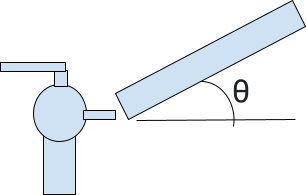
\includegraphics{image2.png}}

        \item [10.] The further the plunger was, the louder and higher pitched the noise.
    \end{itemize}

    \section*{Station 3: Mass on a string}

    \begin{itemize}
        \item [11.]
        
        Easiest to stretch: Shortest spring

        Mediumist to stretch: Long single spring

        Most difficult to stretch: Double spring

        \item [12.]
        
        Lightest: 10 g

        Mediumest: 20 g

        Heaviest: 50 g

        \item [13.] No, it will oscillate slower because most of the kinetic energy that would have been gained from starting higher is not in the system.
        \item [14.] The heaviest weight with the easiest to stretch spring will oscillate the slowest.
        \item [15.] The lightest weight with the hardest to stretch spring will oscillate the fastest.
        \item [16.] \mbox{}\\
        
        \begin{center}
            \begin{tabular}{c | c | c | c}
                Mass & Spring & Time for 10 Oscillations & Natural Frequency (Hz) \\
                \hline
                heavy & easy & 11.40 & 0.878    \\
                heavy & medium & 8.31 & 1.203   \\
                heavy & difficult & 4.75 & 2.105\\
                medium & easy & 7.94 & 1.259    \\
                medium & medium & 5.34 & 1.873  \\
                medium & difficult & 3.22 & 3.106\\
                light & easy & 6.44 & 1.553     \\
                light & medium & 3.75 & 2.667   \\
                light & difficult & 2.16 & 4.629\\
            \end{tabular}
        \end{center}

        \pagebreak

        \item [17.] The lighter the mass, the higher the natural frequency and vice versa.
        \item [18.] The less the spring stretches, the higher the natural frequency and vice versa.
        \item [19.] \mbox{}\\
        
        \begin{center}
            \begin{tabular}{c | c | c | c}
                & Natural frequency depends on: & Adjustments: & Doesn't affect: \\
                \hline
                Air Column & Length and diameter of tube & Decrease length & Diameter   \\
                \hline
                Elastic Band & Mass of the band and tension & decrease mass and tension & ``Fret''   \\
                \hline
                Mass on spring & Mass, spring resistence & Lighter mass, harder spring & Initial displacement   \\
            \end{tabular}
        \end{center}

    \end{itemize}

\end{document}